\documentclass[a4paper,11pt,french]{refart}

\usepackage[utf8]{inputenc}
\usepackage[T1]{fontenc} % LY1 also works
\usepackage{babel}

%% Font settings suggested by fbb documentation.
\usepackage{textcomp} % to get the right copyright, etc.
\usepackage[lining,tabular]{fbb} % so math uses tabular lining figures
\usepackage[scaled=.95,type1]{cabin} % sans serif in style of Gill Sans
\usepackage[varqu,varl]{zi4}% inconsolata typewriter
\useosf % change normal text to use proportional oldstyle figures
%\usetosf would provide tabular oldstyle figures in text
\usepackage{amsthm}
\usepackage{microtype}
\usepackage{listings}
\usepackage{xcolor}

\definecolor{codegreen}{rgb}{0,0.6,0}
\definecolor{codegray}{rgb}{0.5,0.5,0.5}
\definecolor{codepurple}{rgb}{0.58,0,0.82}
\definecolor{backcolour}{rgb}{0.95,0.95,0.92}

\lstdefinestyle{mystyle}{
    backgroundcolor=\color{backcolour},   
    commentstyle=\color{codegreen},
    keywordstyle=\color{magenta},
    numberstyle=\tiny\color{codegray},
    stringstyle=\color{codepurple},
    basicstyle=\ttfamily\footnotesize,
    breakatwhitespace=false,         
    breaklines=true,                 
    captionpos=b,                    
    keepspaces=true,                 
    numbers=left,                    
    numbersep=5pt,                  
    showspaces=false,                
    showstringspaces=false,
    showtabs=false,                  
    tabsize=2
}

\lstset{style=mystyle}

\usepackage{graphicx}
\usepackage{enumitem}
\setlist{leftmargin=*}
\usepackage{listings}
\lstset{basicstyle=\ttfamily,frame=single,xleftmargin=3em,xrightmargin=3em}
\usepackage[os=win]{menukeys}
\renewmenumacro{\keys}[+]{shadowedroundedkeys}
\usepackage{framed}
\usepackage{etoolbox}
\AtBeginEnvironment{leftbar}{\sffamily\small}

\usetikzlibrary{chains,arrows,shapes,positioning}
\usepackage{hyperref}
\hypersetup{
    colorlinks=true,
    linkcolor=blue,
    filecolor=magenta,      
    urlcolor=cyan,
}

\newcommand\AutoCalc{\textsf{Mode d'emploi de PowerUnit}}

\theoremstyle{definition}
\newtheorem{definition}{Définition}[section]

\title{Mode d'emploi de PowerUnit}
\author{HOUEKPETODJI Mahugnon Honoré (\url{homahugnon@gmail.com})\\\url{https://www.linkedin.com/in/mahugnon-honore-4948b6114/}}
\date{\url{https://www.overleaf.com/project/5f5f7a9e37b8f8000181acd7}\\17 Septembre, 2020}
\begin{document}
\maketitle



\tableofcontents
\clearpage

%\section*{Activités }

%\begin{enumerate}
%\item 
%\end{enumerate}

% \begin{tikzpicture}
% \tikzset{every node/.style={on chain,draw,thick,rounded corners,
% minimum height=3em, text width=10em, align=center}}
% \begin{scope}[start chain=going below]
% \node (prepare-group) {Configuration de Power unit };6
% .30+
% \node (import-group) {Écriture du  (\texttt{.xml})};
% \node (enter-rating) {Enter peer ratings given by each student};
% \node (compute-score) {Compute autorated weights and scores};
% \node (export-csv) {Export data for Excel (\texttt{.csv})};
% \end{scope}
% \node[right=of enter-rating] (open-score) {Open previously saved score file (\texttt{.xml})};

% \path[draw,line width=0.4ex, ->,>= angle 60]
% (prepare-group) edge (import-group) 
% (import-group) edge (enter-rating)
% (open-score) edge (enter-rating)
% (enter-rating) edge (compute-score) 
% (compute-score) edge (export-csv);
% \end{tikzpicture}


\section{Généralités sur les tests Unitaires}
\theoremstyle{definition}
\begin{definition}{\textbf{Tester un projet}}
 est un processus manuel ou automatisé qui vise à vérifier qu'un système satisfait les propriétés requises par ses spécifications, ou à détecter les différences entre les résultats produits par le système et ceux attendus par les spécifications
\end{definition}
\subsection{Tests}
\begin{itemize}
    \item préviennent des erreurs introduites par les développeurs;
    \item préviennent des échecs lors d'exécutions;
    \item préviennent des imperfections sur des parties du système susceptibles de causer des échecs d'exécutions;
    \item représentent la \textbf{\textcolor{red}{confiance}} sur l'état de santé du système;
    \item se construisent \textbf{\textcolor{red}{progressivement}}:
    \begin{itemize}
        \item[$\bullet$] pas besoin d'écrire tous les tests d'un coups
        \item[$\bullet$] à chaque nouveau  \textbf{\textcolor{red}{dysfonctionnement ou ticket, écrire des tests}};
    \end{itemize}
    \item c'est d'ailleurs meilleur de les écrire avant d'implémenter la fonctionnalité 
    \begin{itemize}
        \item[$\bullet$] agissent comme les premiers \textbf{\textcolor{red}{clients}} et une meilleure interface; 
    \end{itemize}
    \item représentent une documentation active et synchrone des fonctionnalités présentes dans le système.
    
\end{itemize}
Dans ce guide, nous allons nous concentrer sur les tests unitaires
\subsection{Tests unitaires}
\subsubsection{Vocabulaire}
\theoremstyle{definition}
\begin{definition}{ \textbf{Un cas de test}}
\begin{itemize}
  \item [$\bullet$] est généralement associé à la réussite d'un scénario de cas d'utilisation. Les développeurs ont souvent des scénarios de test à l'esprit, mais ils les réalisent de différentes manières (1) instructions d'affichage; (2) le débuguage ou les fichier de traces; etc.

 \item [$\bullet$] est un ensemble d'entrées de test, de conditions d'exécution et de résultats attendus, développé pour tester un chemin d'exécution particulier. Généralement, le cas est une méthode unique.
 \end{itemize}
 \end{definition}

\begin{definition}{ \textbf{Une suite de test}}
 est une liste de cas de tests liés. La suite peut contenir des routines communes d'initialisation et de nettoyage spécifiques aux cas de tests qu'il contient. Généralement, la suite de test est une classe.
 \end{definition}

\subsubsection{Présentation de cas de test unitaire}
Un cas de test  répond au principe \textbf{\textcolor{red}{Essaie, vérifie, si ça marche}}.
 \begin{figure}[!htp]
  \begin{center}
  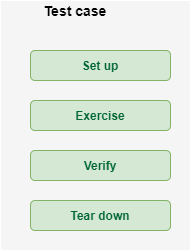
\includegraphics[width=0.5\linewidth]{./testcase.png}
  \caption{Test case}
  \label{fig:testcase}
  \end{center}
\end{figure}
La Figure \ref{fig:testcase}   montre les quatre étapes d'un cas de test unitaire. On distingue:
\begin{itemize}
    \item \textbf{\textcolor{red}{Set up.}} consiste à  préparer les ressources pour le tests;
    \item \textbf{\textcolor{red}{Exercise.}} consiste à exercer la fonctionnalité à tester du  système en tests  sur les ressources précédemment préparées;
    \item \textbf{\textcolor{red}{Verify.}} Consiste à vérifier que le résultat de l'exercice correspond bien au résultat attendu du système en test;
    \item \textbf{\textcolor{red}{Tear down.}} Consiste à libérer les ressources utiliser durant le test
\end{itemize}

\subsubsection{Caractéristiques d'un bon cas test unitaire}
\begin{itemize}
    \item Répétable
\item Pas d'intervention humaine
\item S'auto-décrit
\item Change moins souvent que le système
\item Raconte une histoire
\end{itemize}
\section{Power unit}
\subsection{Présentation}
 \begin{figure}[!htp]
  \begin{center}
  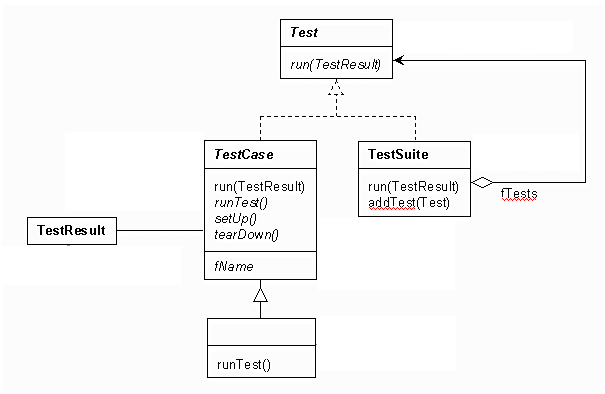
\includegraphics[width=1\linewidth]{./frameworkPBUnit.png}
  \caption{Power unit}
  \label{fig:powerUnit}
  \end{center}
\end{figure}
Power unit est le framework qui permet d'écrire les tests unitaire en Powerbuilder. Il est inspirer de JUnit.
La Figure \ref{fig:powerUnit} presente le diagramme de classe de Power Unit. La classe \textit{\textcolor{red}{TestCase}} est la classe de base pour écrire les tests unitaire en Powerbuilder.  Ainsi tous les tests héritent de la classe  \textit{\textcolor{red}{TestCase}}. 



\subsection{Ecriture de tests avec Power Unit}
Dans le cadre de ce apprentissage, je vais reprendre l'exemple de la documentation de Power Unit.
Le programme que nous allons parcourir résoudra le problème de la représentation de l'arithmétique avec des monnaies multiples. 
 L'arithmétique entre les même monnaies  est triviale ; vous pouvez simplement additionner les deux montants.
 Les choses deviennent plus intéressantes une fois que des monnaies multiples sont introduites. 
 Vous ne pouvez pas vous contenter de convertir une monnaie en une autre pour faire de l'arithmétique puisqu'il n'y a pas de taux de conversion unique.

\subsubsection{Préparation de l'environnement}
Pour suivre ce apprentissage, vous avez besoin:
\begin{itemize}
    \item d'avoir l'IDE \textbf{Powerbuilder} installer sur votre machine
    \item de télécharger les bibliothèques de base de \href{https://github.com/mahugnon/PBUnitBase.git}{ Power Unit}
    \item de télécharger les bibliothèques de l'interface graphique de \href{https://github.com/mahugnon/PBUnitGUI.git}{Power Unit} 
    \item Créer un répertoire qui va accueillir les objets durant ce apprentissage  
    \item Créer un nouvel espace de travail nommé \textit{PBCookBook} 
    \item Créer une \textit{target} nommée \textit{PBCookBook} dans l'espace de travail.
    \item Inclure la bibliothèque \textit{PBUnit.pbl} téléchargée précédemment 
\end{itemize}

 %\menu{File>Save} or pressing \keys{Ctrl+S}.
\subsubsection{Creation d'un objet à tester}
Nous allons commencer par définir simplement un objet  qui représentera une valeur monétaire dans une monnaie unique. 
Mais d'abord, créons un objet de base que nous expliquerons plus loin dans ce mode opératoire:
\begin{itemize}
    \item Créer un nouvel objet de classe \textit{custom class}
    \item Fermez et enregistrez-le sous le nom n\_cst\_MoneyBase dans le PBCookBook.PBL
\end{itemize}
Maintenant, créons l'objet monnaie \textit{money}:
\begin{itemize}
   \item Héritez un nouvel objet de l'objet n\_cst\_MoneyBase
    \item Enregistrez le sous le nom de n\_cst\_Money dans la bibliothèque PBCookBook en lui donnant un commentaire approprié
    \item  Définir deux attributs privés pour la somme et la monnaie \textit{money}

\begin{lstlisting}[language=Python, caption=variable d'instance de n\_cst\_money]
    
        Private Decimal	idc_Amount;
        Private String	is_Currency;

\end{lstlisting}
\item Créer une méthode d'initialisation pour ces attributs lors de leur création

\begin{lstlisting}[language=Python, caption=methode d'initialisation  de n\_cst\_money]
    
    /*	of_Initialize ( decimal adc_Amount, string as_Currency )	*/
    idc_Amount = adc_Amount;
    is_Currency = as_Currency;
    return;
\end{lstlisting}
\item  Créer des accesseurs pour les attributs
\begin{lstlisting}[language=Python, caption=accesseur pour recuperer la somme de l'objet \textit{money}]
    
    /*	of_getAmount (): decimal	*/
return	idc_Amount;

\end{lstlisting}
\begin{lstlisting}[language=Python, caption=accesseur pour recuperer la monnaie de l'objet \textit{money}]
    /*	of_getCurrency ( ): String		*/
    return	is_Currency;
    
\end{lstlisting}
\item  Créez une méthode simple pour ajouter les valeurs de deux objets \textit{money} de la même monnaie et obtenir ainsi un nouvel objet \textit{money}.
\begin{lstlisting}[language=Python, caption=Simple addition de deux montants de la même monnaie]
  /*	of_add(n_cst_money anv_Money):n_cst_Money	*/
n_cst_Money	lnv_Money;

lnv_Money = CREATE n_cst_Money;
lnv_Money . of_Initialize ( THIS.of_getAmount() + anv_Money.of_getAmount(), THIS.of_getCurrency( ));
return	lnv_Money;

\end{lstlisting}
\item Avant de pouvoir procéder, nous avons besoins comparer deux objets \textit{money}.  
Ajoutez une nouvelle méthode of\_Equals() à votre objet \textit{n\_cst\_Money}.
 Deux objets Monnaie sont considérés comme égaux s'ils ont la même monnaie et la même valeur
 
 \begin{lstlisting}[language=Python, caption=Comparaison de deux objets \textit{money}]

 /*	of_equals(n_cst_Money anv_Money):Boolean	*/

 IF IsValid ( anv_Money ) THEN
     return (( anv_Money.of_getAmount() = idc_Amount ) &
         AND ( anv_Money.of_getCurrency() = is_Currency ));
 ELSE
     return false;
 END IF;
 
\end{lstlisting}
\end{itemize}


% \bibliographystyle{plain}
% \bibliography{refs}
\end{document}